\documentclass[UTF8]{article}%z指定文档类型
\usepackage[UTF8]{ctex}%显示中文
\usepackage{graphicx}%引用图包
\usepackage{amsfonts,amsmath,amssymb,amstext,array}%数学相关宏包
\usepackage{xcolor}
\usepackage{hyperref} 
\makeatletter
\renewcommand*\env@matrix[1][*\c@MaxMatrixCols c]{%
\hskip -\arraycolsep
\let\@ifnextchar\new@ifnextchar
\array{#1}}
\makeatother

\begin{document}%文章开始

\title{并行计算}%文章题目
\maketitle% 显示上述标题信息

\newpage
\tableofcontents

\section{矩阵乘并行计算}

\subsection{矩阵基本性质}

\subsubsection{加法}

可交换顺序、可分配可结合、A+(-A)=O

\subsubsection{数乘}

可交换顺序、可分配可结合。

\subsubsection{乘法}

不可交换顺序、可分配可结合。

\subsubsection{转置}

$(A+B)^T=A^T+B^T$

$(kA)^T=kA^T$

$(AB)^T=B^{T}A^T$

$(AT)^T=A$

\subsubsection{共轭}

$(A)_{i,j}=\overline{A_{i,j}}$

矩阵内实部不变,虚部取负。

\subsubsection{注意}

$(A+B)(A+B)=A^2+AB+BA+B^2$

\subsubsection{相关定义}

\begin{itemize}
    \item 行列式:是一个函数,其定义域为det的矩阵A,取值为一个标量,写作det(A)或|A|,A为n×n的正方形矩阵。
    \item 余子式:n阶行列式D中,把元素$a_{oe}$所在的第o行和第e列划去后,留下来的n-1阶行列式叫做元素$a_{oe}$的余子式,记作$M_{oe}$。
    
    k阶余子式:行列式D中划去了k行k列,划去的交叉部分组成子式A(即元素),称剩下的为行列式D的k阶子式A的余子式。

    \item 代数余子式:将余子式$M_{oe}$再乘以-1的o+e次幂记为$A_{oe}$,$A_{oe}$叫做元素$a_{oe}$的代数余子式。
    
    同理k阶代数余子式。此时o、e为行和列的序号累加。
   
    \item 特征值:对于n阶方阵A,如果存在数m和非零n维列向量x,使得Ax=mx成立,则称m是A的一个特征值(characteristic value)或本征值(eigenvalue)。
    \item 特征向量:对于一个给定的线性变换,它的特征向量(本征向量或称正规正交向量)v满足经过该线性变换之后,得到的新向量仍然与原来的v保持在同一条直线上。
    \item 迹:n阶方阵A的对角元素之和称为矩阵A的迹(trace),记作tr(A)。
    \item 正定矩阵:n阶方阵A,如果对任何非零向量z,都有$z^TAz>0$,其中$z^T$表示z的转置,就称M为正定矩阵。大于等于0则为半正定矩阵,小于0则为负定矩阵。
\end{itemize}

\subsubsection{初等变换}

初等变换:设A是m×n矩阵,进行倍乘、互换、倍加行(列)变换,统称为初等变换。包括:

\begin{itemize}
    \item 倍乘:用非零常数k乘A的\textbf{某行(列)}的每个元素。
    \item 互换:互换A的某两行(列)的位置。
    \item 倍加行(列):将A的某行(列)元素的k 倍加到另一行(列)。
\end{itemize}

初等矩阵:单位矩阵经\textbf{一次}初等变换得到的矩阵称为初等矩阵。

等价矩阵:矩阵A经过有限次初等变换变成矩阵B,则称A与B等价(可能有多个矩阵与A等价,其中等价的最简矩阵被称为A的等价标准型)

性质:用初等矩阵P左乘(右乘)A,其结果PA(AP)相当于对A作相应的初等行(列)变换。

\subsection{传分块统方法}

对于矩阵a被分成2×2四块的情况:

$
\begin{bmatrix}
    a_{0,0} & a_{0,1}  \\
    a_{1,0} & a_{1,1}
\end{bmatrix}
$

有:$c_{0,0}=a_{0,0}*b_{0,0}+a_{0,1}*b_{1,0}$

该情况下,每个线程(计算块)中都存储一行A和一列B(矩阵块),(又要传递又要储存)大大增加了存储量,存储量由O(n平方)—>O(n立方)

\subsection{Cannon方法}

该算法在每次计算完成后让计算块内的数据有规律的传递移动,记为M×M矩阵,有:

1. A总体上子块从右往左循环移动1步;$a_{i,j}->a_{i,j-1}$

2. B总体上子块从下往上循环移动1步;$b_{i,j}->b_{i-1,j}$

3. 每个计算块正常相乘,并存入C块中,$c_{i,j}=c_{i,j}+c$;

4. 重复上述过程,累计M次;

最终得到相乘的结果。

\section{线性方程组的并行求解}

\subsection{直接求解法}

\subsubsection{LU分解算法}

对于矩阵形式的线性方程组:Ax=b,如果A满足为方阵且可逆,则A可以被分解为下三角矩阵 L(Lower Triangle Matrix)和上三角矩阵U(Uppder Triangle Matrix)的乘积。即:

PA = LU

得:LUx=Pb

则方程可以被分解为(L)y=(Pb)和(U)x=(y),通过两个相似的步骤依次求解y和x即可。

基本原理是利用高斯消元,原理是在求解方程组Ax=b时将系数矩阵A和右向量b组成增广矩阵,对其进行行的初等变换,最终得到上三角初等矩阵,则自下而上可求得各个x。

在不带入b的情况下,对A矩阵的初等变换操作可以以置换矩阵$E_{ij}$来表示,表示交换第i行和第j行。而此矩阵乘以一个置换矩阵P即可化为下三角形式。

\paragraph{置换矩阵P:}~{}

对于单位矩阵E,交换其内部的行列,即可得到置换矩阵,与矩阵相乘时,对单位矩阵的操作(交换、乘加、乘(但仅交换属于置换矩阵))都会作用到相乘的矩阵上。

\subsubsection{Gauss直接消去}

对矩阵:
$
\begin{bmatrix}
    a_{1,1} & a_{1,2} & ... & a_{1,n}\\
    a_{2,1} & a_{2,2} & ... & a_{2,n}\\
    ...     &                        \\
    a_{m,1} & a_{m,2} & ... & a_{m,n}\\
\end{bmatrix}
$

\begin{itemize}
    \item 从上往下,第二行减去乘以系数$a_{2,1}/a_{1,1}$的第一行:
    
    $a_{2,k}=a_{2,k}-a_{1,k}*a_{2,1}/a_{1,1}$

    更新第二行的值$a_{2,k}$。

    \item 第三行减去乘以系数$a_{3,1}/a_{1,1}$的第一行,减去乘以系数$a_{3,2}/a_{2,2}$的第二行:
    
    $a_{3,k}=a_{3,k}-a_{1,k}*a_{2,1}/a_{1,1}$
    
    $a_{3,k}=a_{3,k}-a_{2,k}*a_{3,2}/a_{2,2}$
    \item 对于第i行的处理,第j列元素有:
    
    \textcolor{red}{$a_{i,j}=a_{i,j}-\sum_{k=1}^{k<i}{(a_{k,j}*a_{i,k}/a_{k,k})}$}  

    第k行乘的因子始终为:$a_{i,k}/a_{k,k}$

    \item 最终得到上三角初等矩阵U。L和P通过反推变换过程可以得到。
    \item 对向量b做相同变换,则可从下而上,逐渐求解出各个未知数。
\end{itemize}

\paragraph{列主元Gauss消去方法:}~{}

\begin{itemize}
    \item 类似于直接方法,但避免了$a_{j,j}$为0时无法消元的情况。将从第j列的$a_{j,j}$及其以下的各元素中选取绝对值最大的元素,然后通过行变换将它交换到主元素$a_{j,j}$的位置上,再进行消元。
    \item 对于第j列,首先找到该列中最大值的所在行l(\textcolor{red}{$l\geq j$即可}),记最大值为$a_{l,j}$。
    \item 然后将第j列第j行即主元$a_{j,j}$的值,与$a_{l,j}$进行对比:
    
    如果$a_{l,j}$等于0就直接退出(该矩阵无法求解);
    
    如果不相等,则将第j行与第l行进行交换,使第j列最大值在主元位置: $swap(a_{l,j},a_{j,j})$。

    \item 对于\textcolor{red}{$i>j$}的每一行i(k表示列),执行操作$a_{ik}=a_{ik}-a_{ik}\times a_{ij}/a_{jj}$,注意j始终指当前的第j列。
    \item 然后依次处理\textcolor{red}{$0\leq j < n$}各列。
\end{itemize}

\subsubsection{Gauss消去并行计算方法}

\begin{itemize}
    \item 并行部分以列为块分割,传递的是因子$f_{i-j}=a_{i,j}/a_{j,j}$(使相邻块加乘相同,表示\textcolor{red}{第i行用的(减去)第j行乘的因子});以及为了定位行的交换,还需要传递最大值所在行l。
    \item 并行部分只计算落在当前线程列区间内的列的因子,并计算区间内列的交换和加乘。
    
    设并行区间为[j0,j1]、行列式为m*m大小。
    
    如果列在区间内:直接计算因子$f_{i-j}$,并向下一个线程发送因子($i\subseteq [j0,j1],j\subseteq [j0+1/j1+1,m]$),(因子\textbf{包括之前线程传来}的,反正传总的就行,没写的也是0)和l。
    
    如果列在区间外(指小于区间),就接受对应列的因子和l。大于也可,反正都是0。

    最终得到区间内需要的所有的因子和l。

    \item 利用因子和l,先按顺序进行所有的列交换,然后按顺序对行加乘运算。最终得到上三角矩阵。
\end{itemize}

\paragraph{三角矩阵的并行求解:}~{}

以下三角矩阵为例:步骤:

$
\begin{bmatrix}
    a_{1,1} & 0       & 0       & ... & 0      \\
    a_{2,1} & a_{2,2} & 0       & ... & 0      \\
    a_{3,1} & a_{2,3} & a_{3,3} & ... & 0      \\
    ...                                        \\
    a_{m,1} & a_{m,2} & a_{m,3} & ... & a_{m,n}\\
\end{bmatrix}
$

% 假设P=3,有:
% 3 i=3   j=0 
% 4       j=1   i+j    i+p-2
% 5       j=2   i+j    i+p-1
% 6 i=6   j=0
% 7       j=1
% 8       j=2
% 9 i=7   j=0

% 11
% 21  22
% 31  32  33
% 41  42  43  44
% 51  52  53  54  55
% 61  62  63  64  65  66
% 71  72  73  74  75  76  77

\begin{itemize}
    \item 并行的部分为列,但出于处理器负载均衡的考虑,每一个并行块并不是相邻的若干列,而是分开的,类似于123,123,123这样的交替排列,每一组大小为P列(等于并行的数量),称为卷帘。
    \item 并行部分原理:从k=0列开始:
    \item 如果属于第一个线程,就使$u_i=b_i$(行$i\subseteq [0,n-1]$),并使$v_i=0$(行$i\subseteq [0,p-2]$)。
    
    否则使$u_i=0$,行范围同上。
    
    (即只在第一个线程处对u赋右值、对v赋初值0)

    \item 判断属于第myid线程,i从myid开始增加,对每一个线程内的第i行(0到p-1),\textcolor{red}{i以p为步长递增},直到最后n:
    
    $for \quad i=myid \quad step \quad p \quad to \quad n-1 $

    \item 在i=0的情况下,不接受数据;否则接收n维向量$v_{recv}$。
    \item 计算$x_k=(u_i+v_0)/a_{ik}$。
    
    \textbf{整个0到p-1只有这一行即k行的x是求的,剩下的由接下来的线程求。}

    \item 更新传入的v向量:
    
    $v_j=v_{j+1}+u_{i+j+1}-a_{i+j+1}*x_k$ , j=0,...,p-3

    $v_{p-2}=u_{i+p-1}-a_{i+p-1}*x_k$ , 类似于j=p-2(改成p-1?)

    \textbf{j在这里指的是每一个i下,对应的行数,随i的变化v向量不断更新。}

    \item 向下一线程发送v向量$v_{send}$。
    \item 更新[i+p,u-1]行范围内的u向量:
    
    $u_j=u_j-a_{jk}*x_k$ , j=i+p,...,n-1

    \item k=K+1。
    \item 继续循环i,最终完成全部求解。\textcolor{red}{每次循环只处理一列!!}
    \item 注意:{
        \begin{itemize}
            \item \textcolor{red}{v用于将本线程的计算结果对接下来的方程的影响传递给其他线程。大小取决于线程总数目。每次循环时都会变化,由新计算出的解来更新。}
            \item 其每次循环计算P次,恰好到下一个本线程之前。
            \item 注意在v的更新中,更新后的$v_0$指的是当前的k对应的k+1行,即迭代更新。但注意其中u(old)的更新同样采用了迭代的方法,在继承下一行$v_j$的同时,有引入了当前线程的u,而最下行的v则\textcolor{red}{并没有添加新的u},也就是说\textcolor{red}{在下次循环到本线程时,v向量所有的u都不是本线程的了},因此在下一次循环到本线程时,计算x时仍然需要加u。(但这样设计是因为v大小只为一个循环的,只能考虑这么多的$a_i*x_i$计算,到下一个循环时需要重新计算$a_{i+p}*x_{i+p}$)
            只含有当前线程计算的全部结果对方程的影响。因此在下一个线程接收到这个数据时,\textcolor{red}{并不包括本线程之前的所得解的影响},因此在x计算公式中可以看到,加上了本线程储存的u(new,用上次计算出的x更新过)。
            \item \textcolor{red}{u表示未计算的所有行方程$d+bx=c-a$中的c-a项,每次计算出一个$x_{k-1}$值后,就会对u进行更新,未解行i的方程(之后的方程)全部减去$x_{k-1}*a_{ik}$}。
            \item u在初始情况下即第一个线程时被初始赋值为b,即为方程右值。
            \item \textcolor{red}{u仅用于标记线程内部所得解对c-a的影响,外部影响必须全部通过传递的v得到。}
        \end{itemize}
    }
\end{itemize}

\subsection{迭代解法}

可以对每一行的方程迭代部分进行划分,每一个计算块处理若干行的迭代方程。

\section{FFT并行算法}

\subsection{复数基本知识}

\begin{itemize}
    \item 复数乘法的在复平面中表现为辐角相加,模长相乘;
    
    即 $(a_1,\theta_1)*(a_2,\theta_2)=(a_1*a_2,\theta_1+\theta_2)$

    \item 单位根:复数w满足$w^n=1$,称为n次单位根。如图所示:
    
    {
        \begin{figure}[htb!]%插入图片
            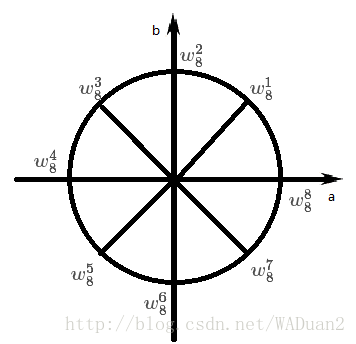
\includegraphics[width=0.4\textwidth]{3-1.png}
        \end{figure}
    }
    
    总n次第m个根记为$w_n^m$,其中n为2的整数倍,则满足性质:

    $w_n^m=-w_n^{m+n/2}$

\end{itemize}

\subsection{快速傅氏变换FFT原理}

\subsubsection{物理意义}

\paragraph{傅里叶变换:}~{}

对于周期函数,是将$f(t)$分解为无数个\textbf{不同频率、不同幅值}的正、余弦信号。用频谱函数表示,自变量是频率$\omega $,因变量是幅值。函数是离散的,自变量都是基频$\omega_0$的整数倍。

对于非周期函数,则是求频谱密度函数,自变量是$\omega $ ,因变量是信号幅值在频域中的分布密度,即单位频率信号的强度。

\textbf{可以将频谱函数和频谱密度函数类比为离散概率分布和概率密度函数。}

\paragraph{快速傅氏变换:}~{}

是离散傅氏变换的快速算法,是对离散傅立叶变换的改进。可用于加速多项式的乘法,将复杂度从$\varTheta(n^2)$优化为$\varTheta(n \log n)$。

\subsubsection{DFT}

对于连续的傅里叶变换,已知:

$F(f)=\int_{-\infty}^{+\infty} f(t) e^{-j 2 \pi f t} d t$

其目的是得到信号的频谱密度函数(t->w(f)),DFT就是t和f都为离散版的傅里叶变换。

由于计算机也只可能计算出有限个频率上对应的幅值密度,因此最终也需要转为离散的情况。转化步骤:

\begin{itemize}
    \item 采样:
    
    利用狄拉克函数的性质:

    $\int_{-\infty}^{\infty} \delta (t-t_0)f(t) \,dx=f(t_0)$

    能够筛选出f(t)在$t_0$时刻的函数值$f(t)$),从而采样$t_0$点,记采样周期为$T_s$,并认为采样附近函数值相等,则f(t)可近似为:

    $f_s=\sum_{n=-\infty}^{\infty}f(t)\delta (t-nT_s) $

    \item 时域离散化:
    
    对采样结果进行傅里叶变换,使时域为无限大求和形式,即:

    $F(\omega )=\sum_{n=-\infty}^{\infty}f(nT_s)e^{-j\omega nT_s}$
    
    \textbf{即每一个$\omega $点的值$F(\omega)$都是由无数个取样点的和组成,且只能得到指定位置的点的值($k\omega$)。}

    \item 频域离散化:
    
    选取有限的N个时刻T,采样间隔同为$T_s$,求和只求范围内的,则可求的k个点的F值为:
    
    $F[k]=\frac{1}{N} \sum_{n=0}^{N-1} f[n] e^{-j \frac{2 \pi}{N} k n}$\qquad k=0,1,2,...,N-1(表示取样点)

    \textcolor{red}{其中$F[k]=F(k\omega_0)T_s=F(\omega_k)T_s$表示频域,}
    
    \textcolor{red}{$f[n]=f(nT_s)=f(t_n)$表示时域。}

    即得到频谱函数$F[k]$,表示的是$k\omega_0$时刻信号幅值大小。

    \item 替代:取样点总数N->n,当前取样点数n->j,复数标志j->i。得:

    $F[k]=\frac{1}{n} \sum_{j=0}^{n-1} f[j] e^{- \frac{2 \pi i j k}{n}}$\qquad k=0,1,2,...,n-1
    
    记\textcolor{red}{$y_k=F(\omega_k)*nT_s$,$x_j=f(t_j)$},则上式可以化为:

    $y_k=\sum_{j=0}^{n-1} x_j e^{- \frac{2 \pi i j k }{n}}$\qquad k=0,1,...,n-1

    \textcolor{red}{k是大循环,j是小循环。}

    \item 注意:该方法的时间复杂度为$\varTheta(n^2)$。
\end{itemize}

\subsubsection{FFT}

用于在DFT的基础上,减少其复杂度。

基本原理:

\begin{itemize}
    \item 记$\omega (n)=e^{-\frac{2 \pi i}{n}}$,则$\omega (n)^k$为方程$x^n=1$的第k根。上式化为:
    
    $y_k=\sum_{j=0}^{n-1} x_j \omega (n)^{kj}$\qquad k=0,1,...,n-1

    \item 同样有性质成立:
    
    性质1:$\omega (n)^{2k}=\omega (n/2)^k$ 不同于:\textcolor{red}{$[\omega (n)^{k}]^2=\omega (2n)^k$}

    性质2:$\omega (n)^{kn}=1$

    性质3:$\omega (n)^{kn/2}=-1$
    
    性质4:$\omega (n)^{k}=\omega (n)^{k+n}=-\omega (n)^{k+n/2}$

    \item 则可利用这些性质化简DFT方程。
    
    把$\omega (n)^{j}$视为整体,首先考虑单个方程的化简。(\textcolor{red}{化简内循环j})
    
    将其拆分成奇数和偶数两部分相加,有:

    $y_{k}=\sum_{j=0}^{n/2-1} x_{2j} \omega(n)^{2jk}+\sum_{j=0}^{n/2-1} x_{2j+1} \omega(n)^{(2j+1)k}$

    记n=2m,利用性质1和4,化简为:

    \textcolor{red}{$y_{k}=\sum_{j=0}^{m-1} x_{2j} \omega(m)^{jk}+\omega(n)^{k}\sum_{j=0}^{m-1} x_{2j+1} \omega(m)^{jk}$}
    
    \item 考虑方程间的化简:(\textcolor{red}{化简大循环k})
    
    由性质4:
    
    $(\omega (m)^{k+m})^j=\omega (m)^{kj}$、$(\omega (n)^{k+m})^j=(\omega (n)^{k+n/2})^j=-\omega (n)^{kj}$

    因此可得$y_{k+m}$的表达式与$y_k$几乎一样,区别仅在于第二部分的$\omega(n)^{k+m}$由于对应方程级数仍然为n,因此变化为$-\omega(n)^{k}$。
    
    最终得到:
    
    $\left\{\begin{array}{l}
        y_{k}=\sum_{j=0}^{m-1} x_{2 j} \omega(m)^{k j}+\omega(n)^{k} \sum_{j=0}^{m-1} x_{2 j+1} \omega(m)^{k j} \\ \\
        y_{k+m}=\sum_{j=0}^{m-1} x_{2 j} \omega(m)^{k j}-\omega(n)^{k} \sum_{j=0}^{m-1} x_{2 j+1} \omega(m)^{k j} \\ \\
        k=0,1, \ldots, m-1
    \end{array}\right.$

    可记为:

    $\left\{\begin{array}{l}
    y_k=G(x^2)+xH(x^2) \\ 
    y_{k+m}=G(x^2)-xH(x^2)
    \end{array}\right.$

    \textcolor{red}{注意其中的x实际上指的是$\omega(m)$,而非前式的x。}
    
    也就是说,只要能够得到$y_k$,就一定能够得到$y_{k+m}$。因为每一个m、k下,H和G总是相等的。

    \item 分治方法:
    
    完整的分治过程\textcolor{red}{不仅包括利用k+m与k的关系不断对方程组进行减半的拆分,还包括对方程内的不同指数的项按奇偶进行拆分}。
    
    对于n=2m的划分可以一直进行下去,但由于每一次方程数目减半,方程内也需要继续进行划分以减少系数,同时每一行y的表达式增加,直到最简单的形式:\textcolor{red}{H和G中不含有x即$y=G+xH$}。
    
    使n=n/2,m=n/2。只对$y_k$处理,然后对G和H分别建立方程$y_{k'}=G(x^2),\quad y_{k''}=H(x^2)$,有$y_{k'}+y_{k''}=y_k$。\textcolor{red}{由于G和H在形式上是完全一样的},因此处理步骤相同。以$y_{k'}$为例,使用$x$替代$x^2$(利用性质1恰好使上一步的$\omega(m)$中的m减小一半,对应新的m),然后就可以按照前文的步骤,将奇部取出x,即$y_{k'}=G'(x^2)+xH'(x^2)$。然后以此类推。

    \item 复杂度:由于对于个点n而言,一共需要在$n^{0.5}$个位置建立方程求解(m对应的位置才需要),而每一次需要进行n次乘法(x与$\omega$相乘),因此总的复杂度量级为$nlog_2(n)$。
    \item 注意:方程数目或多项式系数+1必须为$2^n$次方,否则需要补零。
    \item 注意:可见求解中需要计算全部的$\omega(m)^{kj}$,m=2,4,...,n/2、k=0,1,...,n-1。但利用性质1,k计算到n/2-1就可以了。
\end{itemize}

\subsection{多项式乘法与FFT}

\subsubsection{多项式的表示方法}

系数表示法:用一个多项式的各个项系数来表达该多项式。

点值表示法:把n-1阶多项式看成一个函数,从上面选取n个点,从而利用这n个点来唯一的表示这个函数。每个点记为$(x_i,y(x_i))$。

DFT:多项式由系数表示法转为点值表示法的过程;

IDFT:把一个多项式的点值表示法转化为系数表示法的过程。

\textcolor{red}{FFT就是通过取某些特殊的x的点值来加速DFT和IDFT的过程。}

\subsubsection{点值表示法与FTT关系}

在点值表示法下,单纯的多项式相乘复杂度为$n$,因为在向量乘中,$x_k$保持不变,而仅仅需要将各项$f(x_i)$和$g(x_i)$相乘。

对于DFT和IDFT过程,复杂度则取决于这两个转化过程:$y_i=a_0+a_1*x_i+a_2*x_i^2+...+a_n*x_i^n$方程组,已知A和X向量,求解Y;已知Y和X向量,求解系数向量A。最适合带入的X的值即为方程$x^n=1$的根,$\omega_n^k、k=0,1,..,n-1$。由于每个方程系数是一样的,这样就可以利用之前复数的周期性质,减少乘的数量,快速转化。复杂度同FFT算法,为$nlog_2n$量级。

带入x,对于第k行方程,表示为:

$y_k=\sum_{j = 0}^{n-1} a_jx_k^j = \sum_{j = 0}^{n-1} a_j(\omega_n^k)^j$\qquad k=0,1,...,n-1

参考FFT基本式: $y_k=\sum_{j=0}^{n-1} x_j \omega (n)^{kj}$\qquad k=0,1,...,n-1

则若视$a_j$为$x_j$,则两式完全相等。可以采用同样的方法进行化简。


编写程序时注意($e^{\theta i}=cos(\theta)+isin(\theta)$):对于$\omega_n^k=e^{-{2\pi i k}/n}$,在传统意义上表示时域向频域的转化关系,但在多项式中则表示原项乘以了逆矩阵且扩大了n倍。\textcolor{red}{多项式乘法中,如果只是单纯的相乘,应采用$e^{{2\pi i k}/n}$。}

\subsubsection{FFT加速DFT}

在DFT中,a与x已知,求解y;

\paragraph{基本FFT实现:}~{}

\begin{itemize}
    \item 待乘式次数补0,使满足$n=2^l$;
    \item 计算出所有的x:$\omega(m)^k$、$m=2,4,...,n/2$、$k=0,1,...,n/2-1$。
    \item 利用FFT部分的奇偶分治,只考虑第0行方程,将其拆分到最终只剩两个与$\omega$无关的参数$a$:
    
    即n=1时:$G_0=y_0^{(0)}=a_0*\omega_1^0=a_0$;$H_0=y_1^{(0)}=a_1*\omega_1^0=a_1$。

    \item 然后在纵向和横向上不断“滚雪球”一般累加回各项或方程,顺序与拆分时相反。
    
    {
        \begin{itemize}
            \item 首先考虑横向的累加:
            
            每轮累加时都满足:\textcolor{red}{下一个偶数项/奇数项=上一个偶数项+$\omega_n^k×$上一个奇数项}。其中n是当前方程下的n。
            
            则通过这样的步骤以翻倍的速度不断加回之前被分治的各奇偶项,直到得到最终的y。由于H和G都是一轮一轮累加出来的,避免了利用求和公式累加幂导致j对$\omega$影响。

            \item 然后考虑纵向的累加:
            
            在每一轮横向累加时利用当前n值下的周期性,每一个n下增加对$k+n/2$列的计算即可(即蝴蝶操作)。但注意由于每一次的原方程并不完整,因此每一次纵向回滚时都需要重新计算所有的行方程(更新y)(就是用新的G和H变换加减号来计算)。

        \end{itemize}
    }            
    
    \item 示例:
    
    以8项式为例,首先考虑横向的分治和回滚,略去行系数k:
    
    $x_0$、$x_1$、$x_2$、$x_3$、$x_4$、$x_5$、$x_6$、$x_7$ \qquad n=8
    
    分治步骤:

    第一次:$x_0$、$x_2$、$x_4$、$x_6$;$x_1$、$x_3$、$x_5$、$x_7$ \qquad n=4

    第二次:$x_0$、$x_4$;$x_2$、$x_6$;$x_1$、$x_5$;$x_3$、$x_7$ \qquad n=2

    第三次:$x_0$;$x_4$;$x_2$;$x_6$;$x_1$;$x_5$;$x_3$;$x_7$ \qquad n=1

    回滚:

    最开始:$G_0=a_0$;$H_4=a_4$;$G_2=a_2$;$H_6=a_6$;$G_1=a_1$;$H_5=a_5$;$G_3=a_3$;$H_7=a_7$;\qquad n=1

    滚1次:$G_{04}=G_0+\omega(n)H_4$;$H_{26}=G_2+\omega(n)H_6$;$G_{15}=G_1+\omega(n)H_5$;$H_{37}=G_3+\omega(n)H_7$;\qquad n=2

    滚2次:$G_{0426}=G_{04}+\omega(n)H_{26}$;$G_{1537}=G_{15}+\omega(n)H_{37}$\qquad n=4

    滚3次:$Y=G_{0426}+\omega(n)H_{1537}$\qquad n=8

    得到了最终的y值。

    然后考虑纵向的回滚,记一开始为第0行:
    
    第一次:0->1\qquad n=2,m=1

    第二次:0->2,1->3\qquad n=4,m=2

    第三次:0->4,1->5,2->6,3->7 \qquad n=8,m=4

    最终求得了每一行的y值。

    注意:\textcolor{red}{除非最后一次(n)计算,其他次(n)的计算都是不完整的,因此每一个n下都需要重新计算所有的其余列。}

    \item 递归程序参考:
    
    {
        \begin{figure}[htb!]%插入图片
        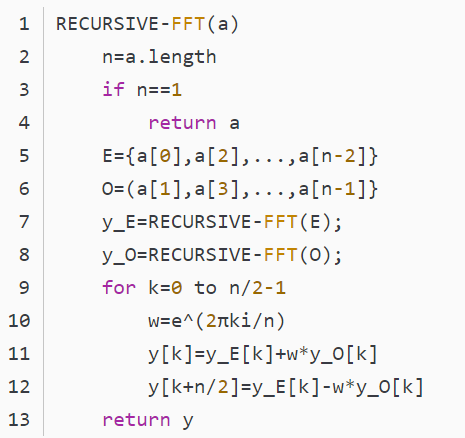
\includegraphics[width=0.5\textwidth]{3-2.png}
        \end{figure}
    }
    
    \item 此过程复杂度为$nlog_2n$。
\end{itemize}

\paragraph{高效FFT实现:}~{}

之前的FFT实现中,在行之间的计算顺序每次(n)都是按0到n增加的,但是行内则是对每一项进行了重新排列,在递归方法下需要花费大量空间用于创建和维护数组。而如果一开始每一行的项就是已经是排列后的,则可以利用迭代法来求解,提高FFT效率。

重要规律:\textcolor{red}{在原始的顺序下,每个项序号用二进制表示(四位),然后把每个数的二进制顺序翻转一下,就是最终拆分完全后每个数的序号。}

蝴蝶变换:输入$x_1$、$x_2$,通过$y_1=x_1+x_2$、$y_2=x_1-x_2$,使最终输出$x_1=y_1$、$x_2=y_2$的方法。

迭代法FFT实现:

\begin{itemize}
    \item 翻转多项式所有的系数$a_i$,变化为需要的排列顺序;
    \item \textcolor{red}{以a的次序为处理顺序;}
    \item 进行主循环,记step,从1开始每次自身乘2递增直到n-1;
    
    (记step个系数的H+xG的值为大单元,则step表示分治下各部分系数数量为step的情况(不管行))
    
    \item 计算当前step下的$\omega_n^1=e^{{2\pi}/n i}$;\textcolor{red}{(由于因为这是逆操作,step始终是只为原来一半的,因此利用当前的H+xG求解新H或G时,在x中需要将step乘2,即$e^{\pi /n i}$)}
    \item 进行中循环,记j,从0开始每次增加2倍的step直到n-1;\textcolor{red}{(将向量a按当前step大小全分割(总计n/step个),每一次循环处理两个大单元(序号间隔step),最终得到全部更新的a向量)}
    
    (j表示当前处理的a向量范围$[j,j+2step)$))

    可以视为对单行方程的分割。随step增加j取值不断减少。当step=n/2时,不分割,对应的$a_j$即j行的计算值。

    \item 进行小循环,记k,从j开始+1增加step个数为止;\textcolor{red}{(利用之前step下计算的上一轮的a向量值,来得到可求的每一行方程内对应传入的step位置的G+xH的值,即更新一部分a向量(2step个))}
    
    (k即表示a向量的序号,每次小循环会更新j即2step的部分a向量,直到全部更新完成)\textcolor{red}{(在第一次传入j中表示行的序号,从0到step;而在之后传入的j下,a向量的序号并不对应于列,需要减去之前的序号(即$k-j$或$k-2*step*l$才表示列))}

    可以视为单方程内分割下的方程间分割的分别计算。随step增加k取值不断增加,当step=n/2时,计算量最大,恰好为全部的a数。

    \item 注意:传入的a矩阵为按顺序排列的系数向量,由于采用了重复赋值更新,在一轮大循环后,a的意义就已经发生变化了,a向量按一定的规律在不同的step下排列,但最后会表示为每一行的累加值。
    \item 程序:
    
    {
        {
        \begin{figure}[htb!]%插入图片
        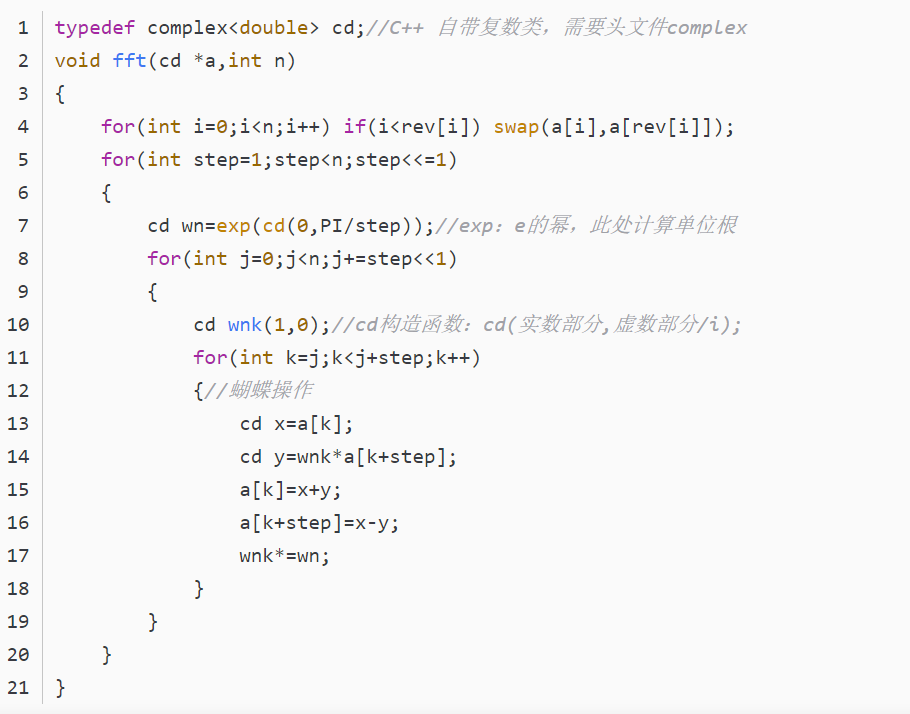
\includegraphics[width=1.0\textwidth]{3-4.png}
        \end{figure}
        }
    }

    \textcolor{red}{注意需要考虑不同行中k的影响,这是通过小循环中从第0行开始,每次循环wnk项乘以一个wn来的($\omega_{2n}^{0+1+1+\dots}$)。}

    \item 蝴蝶变换示意图:
    
    {
        {
        \begin{figure}[htb!]%插入图片
        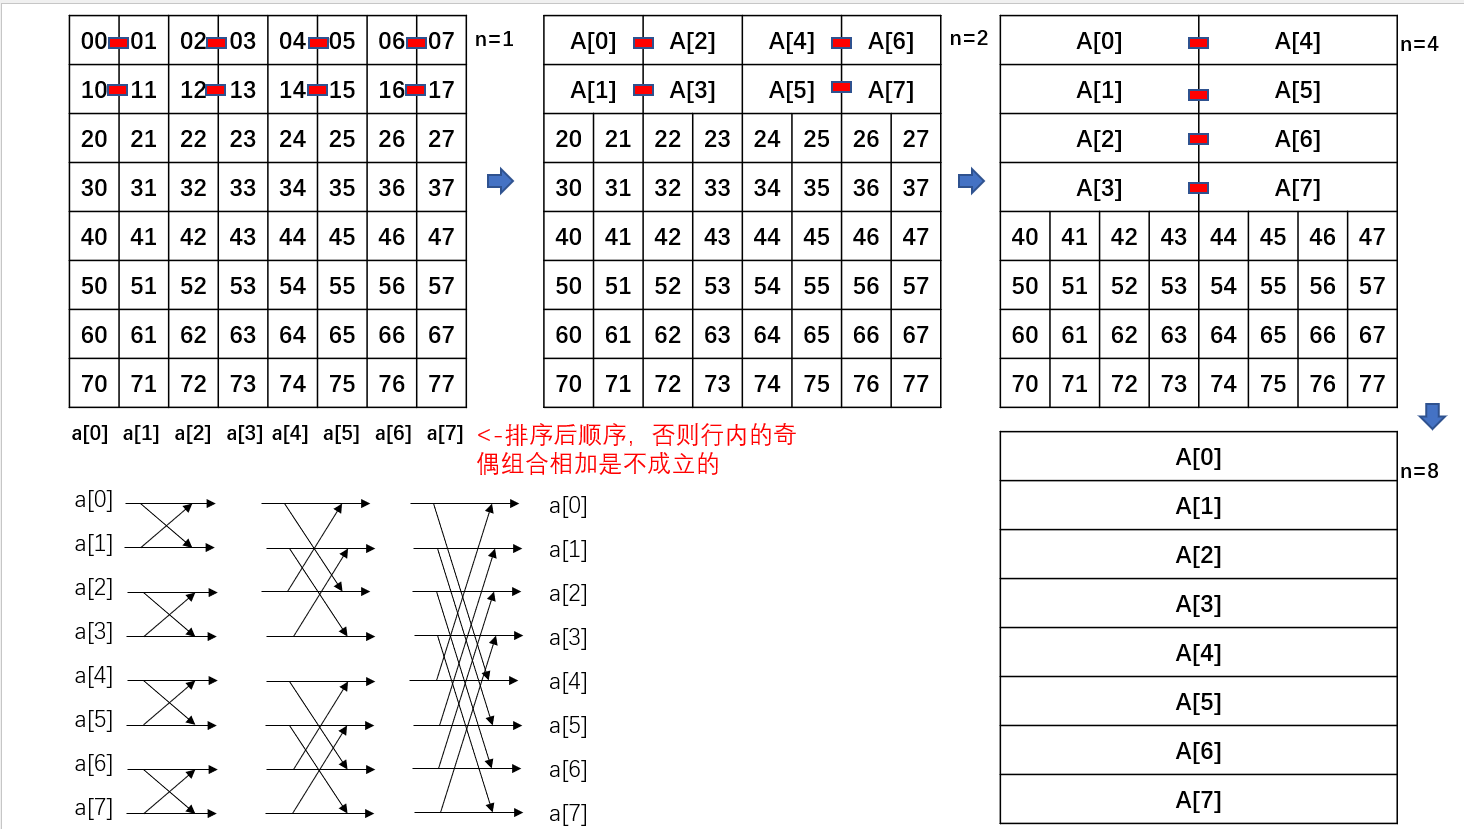
\includegraphics[width=1.0\textwidth]{3-3.png}
        \end{figure}
        }
    }

\end{itemize}

\subsubsection{FFT加速IDFT}

在IDFT中,y与x已知,求解a。

将方程写为如下矩阵形式:(之前也是这种形式,只不过a向量乘进去了)

$\left[\begin{array}{c}y_{0} \\ y_{1} \\ y_{2} \\ y_{3} \\ \vdots \\ y_{n-1}\end{array}\right]=\left[\begin{array}{cccccc}1 & 1 & 1 & 1 & \cdots & 1 \\ 1 & \omega_{n} & \omega_{n}^{2} & \omega_{n}^{3} & \cdots & \omega_{n}^{n-1} \\ 1 & \omega_{n}^{2} & \omega_{n}^{4} & \omega_{n}^{6} & \cdots & \omega_{n}^{2(n-1)} \\ 1 & \omega_{n}^{3} & \omega_{n}^{6} & \omega_{n}^{9} & \cdots & \omega_{n}^{3(n-1)} \\ \vdots & \vdots & \vdots & \vdots & \ddots & \vdots \\ 1 & \omega_{n}^{n-1} & \omega_{n}^{2(n-1)} & \omega_{n}^{3(n-1)} & \cdots & \omega_{n}^{(n-1)^2}\end{array}\right]\left[\begin{array}{c}a_{0} \\ a_{1} \\ a_{2} \\ a_{3} \\ \vdots \\ a_{n-1}\end{array}\right]$

需要在等式两边左侧乘以$\omega$的逆矩阵,即可变为$A=\omega^{-1}y$的格式,与之前的y=ax形式完全一样,可用相同方法求解。即输入为y向量,返回的为新的系数向量a。

可以证明,\textcolor{red}{对于矩阵每一项取倒数再除以n就是该矩阵的逆矩阵}。

注意为保证输出a向量的顺序,也需要在计算前对y向量进行翻转。

则程序基本上与DFT过程相同,\textcolor{red}{区别在于对系数的处理中,将y向量每一项除以n;然后在H+xG处理中,x的初始定义由$\omega_n^k=e^{{2\pi i k}/n}$变为$\omega_n^k=e^{-{2\pi i k}/n}$(e的系数加个负号)}。

完整的程序可以写为一个函数,除上述操作外其他部分完全一样。 

\subsection{二维串行FFT算法}

可以由两个方向的一维FFT来完成。

\section{MPI并行程序设计基础}

\paragraph{与pthread区别}~{}

定义:Massage Passing Interface:是消息传递函数库的标准规范。是一种新的库描述,不是一种语言。

mpi是基于分布式内存系统,而openmp和pthread基于共享内存系统;

即mpi之间的数据共享需要通过消息传递,因为mpi同步的程序属于不同的进程,甚至不同的主机上的不同进程。相反由于openmp和pthread共享内存,不同线程之间的数据就无须传递,直接传送指针就行。

同时mpi不同主机之间的进程协调工作需要安装mpi软件(例如mpich)来完成。


\subsection{并行相关分类}

\paragraph{计算机架构:}~{}

\begin{itemize}
    \item SMP:SMP是对称多处理技术。具有多个CPU,所有的CPU共享一个内存,使用相同的地址空间。所有的CPU通过一条总线(bus)和内存以及IO设备(硬盘等)连接。总线同一时刻只能处理一个请求,当有多个CPU的访存访问请求时,只能一个一个处理。
    \item MMP:类似于集群,但MMP使用了更多定制化的组件,包括网络、处理器、操作系统等;而cluster运行通用操作系统,互连网络使用商业标准的IB和以太网设备连接,存储为SAN、NAS和并行文件系统。
    \item Cluster:集群,它至少将两个系统连接到一起,使两台服务器能够像一台机器那样工作或者看起来好像一台机器。基本特征是具备多个 CPU 模块,每一个CPU模块由多个CPU组成,而且具备独立的本地内存、 I/O 槽口等。
    \item MMP与Cluster区别:
    
    {
        \begin{itemize}
            \item MPP实际上是一台机器,这台机器有使用高速网络紧密连接的成千上万个处理器,只有一个操作系统。
            \item cluster实际上是有多台机器,每个机器有自己的操作系统(一般都是一样的)、硬盘、内存等,这些机器使用一些普通网络的一些变体连接起来,使用某些系统帮助分配任务给这些主机。
        \end{itemize}
    }
\end{itemize}

\paragraph{并行计算机系统结构编程模型(Flynn分类法):}~{}

\begin{itemize}
    \item 单指令单数据(SISD): SISD是标准意义上的串行机,具有如下特点:1)单指令:在每一个时钟周期内,CPU只能执行一个指令流;2)单数据:在每一个时钟周期内,输入设备只能输入一个数据流;3)执行结果是确定的。这是最古老的一种计算机类型。
    \item 单指令多数据(SIMD): SIMD属于一种类型的并行计算机,具有如下特点:1)单指令:所有处理单元在任何一个时钟周期内都执行同一条指令;2)多数据:每个处理单元可以处理不同的数据元素;3)非常适合于处理高度有序的任务,例如图形/图像处理;4)同步(锁步)及确定性执行;5)两个主要类型:处理器阵列和矢量管道。
    \item 多指令单数据(MISD):MISD属于一种类型的并行计算机,具有如下特点:1)多指令:不同的处理单元可以独立地执行不同的指令流;2)单数据:不同的处理单元接收的是同一单数据流。这种架构理论上是有的,但是工业实践中这种机型非常少。
    \item 多指令多数据(MIMD): MIMD属于最常见的一种类型的并行计算机,具有如下特点:1)多指令:不同的处理器可以在同一时刻处理不同的指令流;2)多数据:不同的处理器可以在同一时刻处理不同的数据;3)执行可以是同步的,也可以是异步的,可以是确定性的,也可以是不确定性的。这是目前主流的计算机架构类型。
\end{itemize}

\paragraph{并行程序类型:}~{}

\begin{itemize}
    \item 主从式M-S:即Master/Slaver模式。核心思想是基于分而治之,将一个原始任务分解为若干个语义等同的子任务,并由专门的工作者线程来并行执行这些任务,原始任务的结果是通过整合各个子任务的处理结果形成的。各子任务互不相干。
    \item 对称式SPMD:(Single Program Multiple Data)指单程序多数据。类似于SIMD,但在SPMD中,虽然各处理器并行地执行同一个程序,但所操作的数据不一定相同(即各处理器只在需要时进行同步,而不是同步地执行每一条指令)。
    \item 自主式MPMD:(Single Program Multiple)指多程序多数据。相比于SPMD,相当于各自进程执行各自的程序。SPMD和MPMD的表达能力是相同的,只是针对不同的问题编写难易而已。MPI是可以写SPMD和MPMD的并行程序的。
\end{itemize}

重点在SPMD。

\subsection{并行程序基本结构}

\begin{itemize}
    \item 进入MPI环境。产生通信子(进程序号、进程数)。
    \item 程序主体。
    \item 退出MPI环境。
\end{itemize}

\subsection{MPI数据类型}

\begin{tabular}{l c c c r}
    MPI 数据类型                 &	C中对应数据类型           \\
    MPI\_SHORT                  &	short int               \\
    MPI\_INT	                &   int                     \\
    MPI\_LONG	                &   long int                \\
    MPI\_LONG\_LONG	            &   long long int           \\
    MPI\_UNSIGNED\_CHAR         &	unsigned char           \\
    MPI\_UNSIGNED\_SHORT	    &   unsigned short int      \\
    MPI\_UNSIGNED	            &   unsigned int            \\
    MPI\_UNSIGNED\_LONG	        &   unsigned long int       \\
    MPI\_UNSIGNED\_LONG\_LONG	&   unsigned long long int  \\
    MPI\_FLOAT	                &   float                   \\
    MPI\_DOUBLE	                &   double                  \\
    MPI\_LONG\_DOUBLE	        &   long double             \\
    MPI\_BYTE	                &   char                    \\
\end{tabular}


\subsection{MPI通信子(通信域)基础}

定义及功能:

通信子定义了一组能够互相发消息的进程。在这组进程中,每个进程会被分配一个序号,称作秩(rank),进程间显性地通过指定秩来进行通信。

内容:
\begin{itemize}
    \item 上下文(context):提供了一个相对独立的通信区域,不同的信息在不同的上下文中传递,不同的上下文的信息互不干扰,上下文可以区分不同的通信。
    \item 进程组(group):组是一个进程的有序集合,在实现中可以看作是进程标识符的一个有序集。一个通信域对应一个进程组。
组内的每个进程与一个整数rank相联系,称为序列号,从0开始并且是连续的。
    \item 虚拟处理器拓扑(topology):\dots
\end{itemize}

附注:进程:一个进程对应一个pid号,同一个进程可以属于多个进程组(每个进程在不同进程组中有个各自的rank号),因此也可以属于不同的通信域。

默认(最大范围):MPI\_COMM\_WOLRD,这是MPI已经预定义好的通信子,是一个包含所有进程的通信子。\textcolor{red}{最大集}。

\textbf{通信域产生方法:}

\begin{itemize}
    \item 在已有通信域基础上划分获得:MPI\_Comm\_split
    \item 在已有通信域基础上复制获得:MPI\_Comm\_dup
    \item 在已有进程组的基础上创建获得:MPI\_Comm\_Create
\end{itemize}

\textbf{进程组产生方法:}

可以当成一个集合的概念,可以通过“子、交、并、补”各种方法。所有进程组产生的方法都可以套到集合的各种运算。

\subsection{进程通信原理}

通信的基础建立在不同进程间发送和接收操作。一个进程可以通过指定另一个进程的秩以及一个独一无二的消息标签(tag)来发送消息给另一个进程。接受者可以发送一个接收特定标签标记的消息的请求(也可以不管标签,接收任何消息),然后依次处理接收到的数据。这样的涉及一个发送者以及一个接受者的通信被称作点对点通信。

如果某个进程需要跟所有其他进程通信。则可用专门的接口来处理这类所有进程间的通信,称为集体性通信。

\subsection{MPI基本函数}

\subsubsection{并行环境管理函数}

\paragraph{MPI\_Init(\&argc, \&argv)}~{}

\begin{itemize}
    \item 功能:初始化MPI环境。产生一个通信子(称MPI\_COMM\_WORLD)
    \item 参数:
    {
        \begin{itemize}
            \item 就是C++main函数传入的参数,形式如上。
        \end{itemize}
    }
    \item 备注:必须保证程序中第一个调用的MPI函数是这个函数。不关心返回值。
\end{itemize}

\paragraph{MPI\_Finalize()}~{}

\begin{itemize}
    \item 功能:结束MPI环境。
    \item 参数:无
    \item 备注:任何MPI程序结束时,都需要调用该函数。不关心返回值。
\end{itemize}

\subsubsection{MPI通信子操作函数}

\paragraph{MPI\_Comm\_rank函数}~{}

int MPI\_Comm\_rank(

    \qquad MPI\_Comm comm, //[传入]当前进程所在的通信子

    \qquad int *rank //[传出]进程号

    ) 

\begin{itemize}
    \item 功能:获得当前进程的进程标识(进程号)。
    \item 返回值:不关心。
    \item 备注:在调用该函数时,需要先定义一个整型变量如myid,不需要赋值。将该变量传入函数中,会将该进程号存入myid变量中并返回。
\end{itemize}

\paragraph{MPI\_Comm\_size函数}~{}

int MPI\_Comm\_size(
    
    \qquad MPI\_Comm comm, //[传入](不一定本进程的)通信子。如果通信子为MP\_Comm\_WORLD,即获取总进程数

    \qquad int *size //[传出]进程数目
    
    ) 

\begin{itemize}
    \item 功能:是获取该通信子内的总进程数。
    \item 返回值:不关心。
    \item 备注:用法类似前一个。
\end{itemize}

\paragraph{MPI\_Comm\_dup函数}~{}

int MPI\_Comm\_dup(
    
    \qquad MPI\_Comm comm,//[传入]要复制的通信子

    \qquad MPI\_Comm *newcomm //[传出]新的通信子,具有相同的组和从源复制的任何缓存信息,但它包含新的上下文信息
    
    )

\begin{itemize}
    \item 功能:复制现有通信子及其所有缓存的信息
    \item 返回值:不关心。
    \item 备注:无。
\end{itemize}

\paragraph{MPI\_Comm\_compare函数}~{}

int MPI\_Comm\_compare(
    
    \qquad MPI\_Comm comm1,//[传入]要比较的通信子1

    \qquad MPI\_Comm comm2 //[传入]要比较的通信子2
    
    )

\begin{itemize}
    \item 功能:比较两个通信子
    \item 返回值:
    
    {
        \begin{itemize}
            \item MPI\_IDENT:两个通信子的组和上下文相同。
            \item MPI\_CONGRUENT:上下文不同、组相同。
            \item MPI\_SIMILAR:上下文不同,组的成员相同但次序不同。
            \item MPI\_UNEQUAL:都不相同。
            \item 失败:错误代码。    
        \end{itemize}
    }
    \item 备注:无。
\end{itemize}


\paragraph{MPI\_Comm\_create函数}~{}

int MPI\_Comm\_Create(
    
    \qquad MPI\_Comm comm, //[传入]源通信子

    \qquad MPI\_Group group, //[传入]定义源通信子中请求的进程子集的组

    \qquad MPI\_Comm *newcomm //[传出]新的通信子
    
    )

\begin{itemize}
    \item 功能:提取一组进程的子集,以便在单独的通信子中进行单独的多指令多数据(MIMD)计算。
    \item 返回值:返回成功时为MPI\_SUCCESS,否则为错误代码。
    \item 备注:创建新的,老的还在。group需要自己定义。
\end{itemize}

\paragraph{MPI\_Comm\_split函数}~{}

int MPI\_Comm\_split(

    \qquad MPI\_Comm comm,//[传入]要拆分的通信子。也就是被划分的范围

    \qquad int color,//[传入]相同的color的通信子会被划分成同一个子通信子

    \qquad int key,//[传入]新通信子中调用进程的相对等级(rank)。进程在新的通信子中按参数键的值定义的顺序排列
    
    \qquad \_Out\_ MPI\_Comm *newcomm //[传出]新的通信子

    )

\begin{itemize}
    \item 功能:用于将指定的单个通信的进程组划分为任意数量的子组。
    \item 返回值:返回成功时为MPI\_SUCCESS,否则为错误代码。
    \item 备注:将原有的通信子拆分了,新的组成老的。且子组的数量由在所有进程中指定的color数量确定。生成的通信器不重叠。
\end{itemize}

\paragraph{MPI\_Comm\_free函数}~{}

int MPI\_Comm\_free(
    
    \qquad MPI\_Comm *comm //[输入]指向要释放的通信子的指针

);

\begin{itemize}
    \item 功能:释放通过dup、create或split创建的通信子。
    \item 返回值:成功时返回MPI\_SUCCESS,否则返回错误代码。
    \item 备注:
    
    此操作将通信子标记为释放。句柄设置为MPI\_COMM\_NULL。任何使用此通信子的挂起操作都将正常完成。直到没有对对象的活动引用时,对象才会被释放。

    这一功能既适用于内部通信子,也适用于外部通信子。
    
    所有缓存属性的删除被回调函数以不确定的顺序调用。

\end{itemize}

\section{点到点通信函数}

\subsection{阻塞式}

阻塞式:发送或接受完数据后该rank进程才会继续执行。而且必须发送成功(但不一定接收成功)。

\subsubsection{MPI\_Send函数}

int MPI\_Send(

    \qquad void* data,//[传入]发送缓冲区地址(要发送数据的所在地址)

    \qquad int count,//[传入]要发送数据的大小

    \qquad MPI\_Datatype datatype,//[传入]数据的类型

    \qquad int dest,//[传入]目标的进程编号

    \qquad int tag,//[传入]消息标记(用于区分不同类型的消息)

    \qquad MPI\_Comm send\_comm//[传入]目标的通信子
    
    )

\begin{itemize}
    \item 功能:执行标准模式发送操作,并在可以安全地再利用发送缓冲区时返回(直到缓存为空)。
    \item 返回值:成功时返回MPI\_SUCCESS,否则返回错误代码。
    \item 备注:为非本地函数,成功完成取决于是否存在匹配的接收函数。
\end{itemize}

\subsubsection{MPI\_Recv函数}

int MPI\_Recv(

    \qquad void            *buf,//[传出]接收缓冲区地址(要接收数据的存放地址)

    \qquad int             count,//[传入]接收的数据大小

    \qquad MPI\_Datatype   datatype,//[传入]数据的类型

    \qquad int             source,//[传入]指定来源的进程编号,若为MPI\_ANY\_SOURCE表示任意来源

    \qquad int             tag,//[传入]指定来源的消息标记,若为MPI\_ANY\_TAG表示任意标签都接受

    \qquad MPI\_Comm       recv\_comm,//[传入](接收方)通信子,需要与send中的相同。通常情况下send和recv均为MPI\_COMM\_WOLRD

    \qquad MPI\_Status      *status //[传出]接受状态,即指向描述已完成操作的MPI\_Status对象(结构体)的指针。如果不需要该状态信息,直接赋常量MPI\_STATUS\_IGNORE即可

);

\begin{itemize}
    \item 功能:执行接收操作,并且在收到匹配的消息之前不返回(直到缓存被填充)。
    \item 返回值:成功时返回MPI\_SUCCESS,否则返回错误代码。
    \item 备注:
    
    {
        \begin{itemize}
            \item 接收消息的长度必须小于或等于接收缓冲区的长度。如果所有传入数据都不适合接收缓冲区,则此函数将返回溢出错误。
            \item 发送和接收操作之间存在不对称性。接收操作可以接受来自任意发送方的消息,但发送操作必须指定唯一的接收方。
            \item 注意防止死锁。
        \end{itemize}
    }

\end{itemize}

\paragraph{函数成功接受的必要条件}~{}

\begin{itemize}
    \item \textcolor{red}{send\_comm==recv\_comm(都是要为接收方的通信子)}
    \item \textcolor{red}{send\_tag==recv\_tag}
    \item \textcolor{red}{send\_dest==recv\_rank(接收方进程编号)}
    \item \textcolor{red}{send\_rank(发送方进程编号)==recv\_source}
\end{itemize}

\subsubsection{MPI\_Sendrecv合成函数}

int MPI\_Sendrecv(
  
    \qquad void         *sendbuf,//[传入]发送缓冲区地址
    
    \qquad int          sendcount,//[传入]数据大小

    \qquad MPI\_Datatype sendtype,//[传入]信息的数据类型

    \qquad int          dest,//[传入]目标的进程编号

    \qquad int          sendtag,//[传入]消息标记

    \qquad void         *recvbuf,//[传出]接收缓冲区地址

    \qquad int          recvcount,//[传入]接收的数据大小

    \qquad MPI\_Datatype recvtype,//[传入]指定来源的数据类型

    \qquad int          source,//[传入]指定来源(接收)的进程编号

    \qquad int          recvtag,//[传入]指定来源的消息标记

    \qquad MPI\_Comm     comm,//[传入](接收方)通信子

    \qquad MPI\_Status   *status//[传出]接受状态,同上

);

\begin{itemize}
    \item 功能:发送和接收消息。
    \item 返回值:成功时返回MPI\_SUCCESS,否则返回错误代码。
    \item 备注:send、recv、sendrecv互相兼容,sendrecv既可以接受send的数据,也可以给recv发送数据。
\end{itemize}

\subsubsection{MPI\_Sendrecv\_Replace合成函数}

int MPI\_Sendrecv\_replace(

    \qquad void* buffer,//[传入传出]发送和接收缓冲区的初始地址

    \qquad int count,//[传入传出]数据的大小

    \qquad MPI\_Datatype sendtype,//[传入传出]数据的类型

    \qquad int dest,//[传入]目标的进程编号rank

    \qquad int sendtag,//[传入]发送的信息的消息标记

    \qquad int source,//[传入]指定来源的进程编号

    \qquad int recvtag,//[传入]指定来源的消息标记

    \qquad MPI\_Comm comm,//[传入](接收方)通信子

    \qquad MPI\_Status*status//[传出]接受状态,同上

)

\begin{itemize}
    \item 功能:使用单个缓冲区发送和接收消息。
    \item 返回值:成功时返回MPI\_SUCCESS,否则返回错误代码。
    \item 备注:与Sendrecv相比,不同之处在于使用同一个缓冲区来接收和发送数据(因此前三个参数是一样的)。也正因为如此,效率相比于Sendrecv低下。
\end{itemize}

\subsubsection{消息查询函数MPI\_Probe}

int MPI\_Probe(

    \qquad int         source,//[传入]查询的进程编号

    \qquad int         tag,//[传入]查询的消息标记

    \qquad MPI\_Comm   comm,//[传入]查询的通信子

    \qquad MPI\_Status *status//[传出]接受状态,同上

);

\begin{itemize}
    \item 功能:探测接收消息的内容,但不影响实际接收到的消息。
    \item 返回值:函数执行成功时返回MPI\_SUCCESS,否则返回错误代码。
    \item 备注:为阻塞型探测,直到有一个符合条件的消息到达才返回,\textbf{即函数成功返回则一定接收到了信息}。
\end{itemize}

\subsubsection{消息查询函数MPI\_IProbe}

int MPI\_IProbe(

    \qquad int         source,//[传入]查询的进程编号

    \qquad int         tag,//[传入]查询的消息标记

    \qquad MPI\_Comm   comm,//[传入]查询的通信子

    \qquad int         *flag,//[传出]标记,如果找到了符合要求的信息(source、tag、comm),就为1,否则为0

    \qquad MPI\_Status *status//[传出]接受状态,同上

);

\begin{itemize}
    \item 功能:同Probe,但为非阻塞型。
    \item 返回值:函数执行成功时返回MPI\_SUCCESS,否则返回错误代码。
    \item 备注:为非阻塞型探测,无论是否有一个符合条件的消息到达,都立刻返回。通过flag判断是否找到。
\end{itemize}

\subsubsection{消息查询函数MPI\_Get\_Counte}

int MPI\_Get\_count(

    \qquad MPI\_Status   *status,//[传出]接收状态

    \qquad MPI\_Datatype datatype,//[传入]每个接收缓冲区元素的数据类型

    \qquad int          *count//[传出]接收到的元素数目

);

\begin{itemize}
    \item 功能:获得接收到的某一种类型的元素数量。
    \item 返回值:成功时返回MPI\_SUCCESS,否则返回错误代码。
    \item 备注:通过对count的值进行修改。
\end{itemize}

\subsection{非阻塞式}

\paragraph{非阻塞式(异步通信)与阻塞式(同步通信)区别}

\begin{itemize}
    \item 同步通信中在接受到数据和发送完数据之前,进程处于挂起状态,完成后才允许进程继续执行下一语句。
    \item 异步通信中发送方在将要发送的消息在消息缓冲区中后,即可返回;接受方不管消息缓冲区中是否已有发送原语发送的消息,都将返回。当消息被确切地发出或收到时,系统将用中断信号(非阻塞式会产生独有的句柄request)通知发送方或接受方。在此之前,它们可以周期性地查询、暂时挂起或执行其它计算,以实现计算与通信的重叠。
    \item 异步通信需要系统提供一个消息缓冲区,同步通信则不需要。
    \item 在同步通信中,通信可以是异步开始的,但必将是同步结束的;在异步通信中,通信可以是异步开始的,也可以是异步结束。
\end{itemize}

\subsubsection{MPI\_Isend函数}

int MPI\_Isend(

    \qquad void*                data,//[传入]发送缓冲区地址

    \qquad int                  count,//[传入]数据大小

    \qquad MPI\_Datatype        datatype,//[传入]信息的数据类型

    \qquad int                  dest,//[传入]目标的进程编号

    \qquad int                  tag,//[传入]消息标记(用于区分不同类型的消息)

    \qquad MPI\_Comm            send\_comm,//[传入]目标的通信子

    \qquad MPI\_Request         *request //[传出]\textcolor{red}{所请求的通信操作的句柄},用来描述非阻塞发送或接收的完成情况。是提供给后面的非阻塞通信检测/等待函数用的。
    
    )

\begin{itemize}
    \item 功能:启动标准模式发送操作,在调用后不用等待通信完全结束就可以返回。
    \item 返回值:成功时返回MPI\_SUCCESS,否则返回错误代码。
    \item 备注:本地函数,此函数可以在将消息发送到缓冲区之前返回。\textcolor{red}{也就是说,在执行完该函数后,数据并没有完全写入缓冲区就已经开始执行接下来的命令了,并不会阻塞在这里等待发送完成,}因此函数返回后不能立刻修改data中的内容,否则发送的数据也跟着变化,需要执行消息请求完成函数MPI\_Wait保证发送完毕。
\end{itemize}

\subsubsection{MPI\_Irecv函数}

int MPI\_Irecv(

    \qquad void            *buf,//[传出]接收缓冲区地址

    \qquad int             count,//[传入]接收的数据大小

    \qquad MPI\_Datatype   datatype,//[传入]信息的数据类型

    \qquad int             source,//[传入]指定来源的进程编号,若为MPI\_ANY\_SOURCE表示任意来源

    \qquad int             tag,//[传入]指定来源的消息标记,若为MPI\_ANY\_TAG表示任意标签都接受

    \qquad MPI\_Comm       recv\_comm,//[传入](接收方)通信子,需要与send中的相同。通常情况下send和recv均为MPI\_COMM\_WOLRD

    \qquad MPI\_Status     *status,//[传出]接受状态,即指向描述已完成操作的MPI\_Status对象(结构体)的指针。如果不需要该状态信息,直接赋常量MPI\_STATUS\_IGNORE即可

    \qquad MPI\_Request    *request//[传出]\textcolor{red}{所请求的通信操作的句柄},同之前

);

\begin{itemize}
    \item 功能:执行接收操作,在调用后不用等待通信完全结束就可以返回。
    \item 返回值:成功时返回MPI\_SUCCESS,否则返回错误代码。
    \item 备注:此函数是本地的。此函数可以在将消息接收到缓冲区之前返回。\textcolor{red}{即该函数返回后,数据同样并没有写入完全缓冲区,接收并没有完成,}同样需要执行消息请求完成函数MPI\_Wait保证接收完毕后才能操作这部分数据。
    \item 在调用wait和test后,已经完成的通信操作的句柄request将不可用。
\end{itemize}

\subsubsection{消息请求完成函数MPI\_Wait}

int MPI\_Wait(

    \qquad MPI\_Request *request,//[传入]通信对象的句柄

    \qquad MPI\_Status  *status//[传出]接收状态,同之前

);

\begin{itemize}
    \item 功能:用于等待MPI请求完成。
    \item 返回值:功时返回MPI\_SUCCESS,否则返回错误代码。
    \item 备注:
    
    {
        \begin{itemize}
            \item \textbf{此函数成功返回时,表示request指针表示的通信操作完成,否则通信操作函数就不会结束。}\textcolor{red}{也就是说程序会卡住直到函数执行完毕}。
            \item 用于一个非阻塞通信。
            \item 非本地操作,成功完成可能取决于其他进程的匹配操作,即一直等到相应的通信完成后才成功返回。
            \item 通信操作为空时,立即返回空状态。
            \item 往往与isend和irecv连用,与阻塞式区别在于程序在执行到通信时会不会挂起。
            \item 若接收消息的进程先接收、发送消息的进程再发送,则MPI就只会填充程序提供的缓冲区(发送,接收缓冲区)。而无需使用MPI提供的消息缓冲区。这可以减少在接收进程端的内存拷贝操作,提高性能。
        \end{itemize}
    }

\end{itemize}

\subsubsection{消息请求完成函数MPI\_Waitany}

int MPI\_Waitany(

    \qquad int         count,//[传入]通信对象的数目

    \qquad MPI\_Request *array\_of\_requests,//[传入](未完成的)通信对象句柄的数组指针:定义为MPI\_Request request[count]

    \qquad int         *index,//[传出]指向一个整数的指针,整数表示通信完成的通信对象在数组中的索引

    \qquad MPI\_Status  *status//[传出]接受状态

);

\begin{itemize}
    \item 功能:用于等待非阻塞通信对象数组中的任意一个通信对象的完成。当存在多个通信对象时,一旦有一个通信完成,就返回该通信所对应通信对象的序号index,并释放该通信对象,并把该通信的相关信息存放在status中。
    \item 返回值:功时返回MPI\_SUCCESS,否则返回错误代码。
    \item 备注:
    
    注意区分*request和*array\_of\_requests:

    {
        \begin{itemize}
            \item *request:\textcolor{red}{指的是单个通信对象句柄的地址,调用时传入$\&$,同Ised和Irecv。}
            \item *array\_of\_requests:\textcolor{red}{指的是通信对象的集合,调用时传入集合即数组的名字。}
        \end{itemize}
    }

    注意区分*index和*array\_of\_index:
    
    {
        \begin{itemize}
            \item *index:\textcolor{red}{在wait、waitany这种输出为1个通信对象的情况下,地址为该通信对象在数组中的编号;}
            \item *array\_of\_index:\textcolor{red}{在waitsome这种输出为多个通信对象的情况下,为数组指针,表示第I个通信对象对应的通信完成信息存放在array\_of\_statuses[I]中,其中完成为1,未完成为0;}
            \item waitall中没有index。
        \end{itemize}
    }

\end{itemize}

\subsubsection{消息请求完成函数MPI\_Waitall}

int MPI\_Waitall(

    \qquad int         count,//[传入]通信对象的数目

    \qquad MPI\_Request *array\_of\_requests,//[传入]通信对象句柄的数组指针

    \qquad MPI\_Status  *array\_of\_statuses//[传出]接受状态

);

\begin{itemize}
    \item 功能:用于等待非阻塞通信对象数组中的所有通信对象的完成。当所有的通信完成时才返回,并释放所有的通信对象。
    \item 返回值:功时返回MPI\_SUCCESS,否则返回错误代码。
    \item 备注:无。
\end{itemize}

\subsubsection{消息请求完成函数MPI\_Waitsome}

int MPI\_Waitsome(

    \qquad int         incount,//[传入]通信对象的数目

    \qquad MPI\_Request *array\_of\_requests,//[传入]通信对象句柄的数组指针

    \qquad int         outcount,//[传出]信完成的通信对象的数量

    \qquad int         *array\_of\_index,//[传出]数组指针,表示通信完成的全部通信对象在数组中的索引

    \qquad MPI\_Status  *array\_of\_status//[传出]接受状态

);

\begin{itemize}
    \item 功能:用于等待非阻塞通信对象数组中的任意数量的通信对象的完成。当任意数目的通信完成时就返回,并释放通信完成的通信对象。
    \item 返回值:功时返回MPI\_SUCCESS,否则返回错误代码。
    \item 备注:完成非阻塞通信的数目记录在outcount中,相应的非阻塞通信对象的下标存放在下标数组中,对应通信的相关信息存放在array\_of\_statuses中。
\end{itemize}

\subsubsection{消息请求检查函数MPI\_Test}

\textbf{test与wait区别:}

\begin{itemize}
    \item wait要一直等到相应的非阻塞通信完成后才成功返回,而test在调用后会立刻返回。
    \item wait在any、some的情况下,会给出具体的完成的通信对象的编号;而test在any的情况下则不会,只会给出当前是否满足通信完成的判断,仅some情况下给出编号。
    \item 相比于wait中的index指示完成的通信对象的编号,在test中用flag来取代,仅用于判断是否满足要求。
\end{itemize}

int MPI\_Test(

    \qquad MPI\_Request  *request,//[传入]通信对象句柄的指针

    \qquad int           *flag,//[传出]指示请求是否已完成的判断指针,通信完成为1,否则为0

    \qquad MPI\_Status   *status//[传出]接受状态

);

\begin{itemize}
    \item 功能:用于测试非阻塞通信中通信完成的情况,立即返回。
    \item 返回值:功时返回MPI\_SUCCESS,否则返回错误代码。
    \item 备注:函数执行后立刻返回,不会等待。
\end{itemize}

\subsubsection{消息请求检查函数MPI\_Testany}

int MPI\_Testany(

    \qquad int           count,//[传入]通信对象的数目

    \qquad MPI\_Request  *request,//[传入]通信对象句柄的数组指针

    \qquad int           *flag,//[传出]指示请求是否已完成的判断指针,对应索引位置的通信完成则为1,否则为0

    \qquad MPI\_Status   *status//[传出]接受状态
    
);

\begin{itemize}
    \item 功能:用于测试非阻塞通信数组中是否有任何一个对象已经完成,若有对象完成\textbf{(若有多个,任取一个)},令flag=1立即返回,并释放该对象;否则令flag=0并立即返回。
    \item 返回值:功时返回MPI\_SUCCESS,否则返回错误代码。
    \item 备注:如果调用时没有完成的通信,flag仍然为0。
\end{itemize}

\subsubsection{消息请求检查函数MPI\_Testall}

int MPI\_Testall(

    \qquad int           count,//[传入]通信对象的数目

    \qquad MPI\_Request  *request,//[传入]通信对象句柄的数组指针

    \qquad int           *flag,//[传出]指示请求是否已完成的判断指针,全部通信完成则为1,否则为0

    \qquad MPI\_Status   *status//[传出]接受状态
    
);

\begin{itemize}
    \item 功能:当非阻塞通信数组中有任意一个非阻塞通信对象对应的非阻塞通信没有完成时,令flag=false并立即返回;当所有通信都已经完成时,令flag=true并立即返回。
    \item 返回值:功时返回MPI\_SUCCESS,否则返回错误代码。
    \item 备注:无。
\end{itemize}

\subsubsection{消息请求检查函数MPI\_Testsome}

int MPI\_Testsome(

    \qquad int           incount,//[传入]通信对象的数目

    \qquad MPI\_Request  *request,//[传入]通信对象句柄的数组指针

    \qquad int           outcount,//[传出]通信完成的通信对象的数目

    \qquad int           *array\_of\_indices,//[传出]数组指针,表示通信完成的全部通信对象在数组中的索引

    \qquad MPI\_Status   *status//[传出]接受状态
    
);

\begin{itemize}
    \item 功能:立即返回,有几个非阻塞通信已经完成,就令outcount等于几,且将完成对象的下标记录在数组中。若没有非阻塞通信完成,则返回outcount=0。
    \item 返回值:功时返回MPI\_SUCCESS,否则返回错误代码。
    \item 备注:\textbf{此函数没有flag判断参数,是通过outcount参数是否为0来发挥原flag作用的。}
\end{itemize}

\subsection{持久通讯}

\subsubsection{消息请求检查函数MPI\_Send\_init}

int MPI\_Send\_init(

    \qquad void         *buf,//[传入]发送缓冲区地址

    \qquad int          count,//[传入]数据大小

    \qquad MPI\_Datatype datatype,//[传入]信息的数据类型

    \qquad int          dest,//[传入]目标的进程编号

    \qquad int          tag,//[传入]消息标记

    \qquad MPI\_Comm     comm,//[传入]目标的通信子

    \qquad MPI\_Request  *request//[传出]所请求的通信操作的句柄,同之前

);

\begin{itemize}
    \item 功能:执行发送操作,但请求是持久的,即产生的通信句柄可以重复使用,但每次使用时需要激活和取消占用。
    \item 返回值:成功时返回MPI\_SUCCESS,否则返回错误代码。
    \item 备注:如果另外一个通信在一个并行计算的内部循环中不断地以\textbf{同样的参数}被执行,则没必要每次重新创建通信句柄,即可把这些通信参数一次性捆绑到一个持久通信请求,然后不断用该请求初始化(激活)和释放(取消占用)消息。
    \item 注意:\textbf{在激活的区间内,该通信就等于一个非阻塞通信}。
    
    \textbf{释放有两种方法,一种是free释放,另一种是wait或者test成功返回,且不可以同时采用。}
\end{itemize}

\subsubsection{MPI\_Recv\_init函数}

int MPI\_Recv\_init(

    \qquad void            *buf,//[传出]接收缓冲区地址

    \qquad int             count,//[传入]接收的数据大小

    \qquad MPI\_Datatype   datatype,//[传入]信息的数据类型

    \qquad int             source,//[传入]指定来源的进程编号,若为MPI\_ANY\_SOURCE表示任意来源

    \qquad int             tag,//[传入]指定来源的消息标记,若为MPI\_ANY\_TAG表示任意标签都接受

    \qquad MPI\_Comm       recv\_comm,//[传入](接收方)通信子,需要与send中的相同。通常情况下send和recv均为MPI\_COMM\_WOLRD

    \qquad MPI\_Request  *request//[传出]所请求的通信对象的句柄

);

\begin{itemize}
    \item 功能:执行接收操作,但请求是持久的,同样需要激活和取消占用。
    \item 返回值:成功时返回MPI\_SUCCESS,否则返回错误代码。
    \item 备注:同上可用于化简接收循环。
\end{itemize}

\subsubsection{MPI\_Start函数}

int MPI\_Start(

    \qquad MPI\_Request *request //[传入]通信对象的句柄

);

\begin{itemize}
    \item 功能:激活持久通信产生的句柄request所对应的通信。
    \item 返回值:成功时返回MPI\_SUCCESS,否则返回错误代码。
    \item 备注:每次使用持久通信对象时都需要执行。
\end{itemize}

\subsubsection{MPI\_Startall函数}

int MPI\_Startall(

    \qquad int          count,//[传入]通信对象的数目

    \qquad MPI\_Request *array\_of\_requests, //[传入]通信对象的句柄的数组指针

);

\begin{itemize}
    \item 功能:激活持久通信产生的句柄所对应的通信集合。
    \item 返回值:成功时返回MPI\_SUCCESS,否则返回错误代码。
    \item 备注:每次使用持久通信对象时都需要执行。
\end{itemize}

\subsubsection{MPI\_Request\_free函数}

int MPI\_Request\_free(

    \qquad MPI\_Request *requests, //[传入]通信对象的句柄

);

\begin{itemize}
    \item 功能:释放通信对象(及所占用的内存资源)。
    \item 返回值:成功时返回MPI\_SUCCESS,否则返回错误代码。
    \item 备注:每次使用的持久通信对象完毕时都需要执行。只能一个一个的释放。
    
    \textbf{若该通信请求相关联的通信操作尚未完成,则等待通信的完成再返回,因此通信请求的释放并不影响该通信的完成。}

    该函数成功返回后request被置为MPI\_REQUEST\_NULL,与wait、test类似。

\end{itemize}

\subsubsection{MPI\_Cancel函数}

int MPI\_Cancel(

    \qquad MPI\_Request *request //[传入]通信对象的句柄

);

\begin{itemize}
    \item 功能:非阻塞型,用于取消一个尚未完成的通信请求。
    \item 返回值:成功时返回MPI\_SUCCESS,否则返回错误代码。
    \item 备注:原理是在MPI系统中设置一个取消该通信请求的标志后立即返回,具体的取消操作由MPI系统在后台完成。
    
    \textbf{若相应的通信请求已经开始,则它会正常完成,不受取消操作的影响;若相应的通信请求还没开始,则可以释放通信占用的资源。}

    \textcolor{red}{仍需用MPI\_WAIT,MPI\_TEST或MPI\_REQUEST\_FREE来释放该通信请求。}

\end{itemize}

注意:\textcolor{red}{free和cancel都是针对非阻塞通信的,用于结束它们(前者释放后者取消)。}

\subsubsection{MPI\_Test\_cancelled函数}

int MPI\_Test\_cancelled(

    \qquad MPI\_Status *status,//[传入]接收状态

    \qquad int         *flag //[传出]通信对象通信情况,1表示请求成功被取消,否则为1

);

\begin{itemize}
    \item 功能:测试以查看请求是否已取消。
    \item 返回值:成功时返回MPI\_SUCCESS,否则返回错误代码。
    \item 备注:传入的为接受状态,想调用此函数不可将接受状态设置为不需要。此函数往往和MPI\_Cancel函数联用以查看取消情况。
\end{itemize}

\subsection{高维进程}

通常先定义一组按顺序序号从小到大的行通信子,然后利用MPI\_Comm\_split函数对每个通信子进行拆分,从而产生列通信子,最终组成二维进程。

方法:在定义行通信子内将传入进程的color按一定的规律赋予不同的color值用于将进程划分给不同的通信子、以及赋予不同的key值用于指定进程在通信子内的优先级,然后利用split函数划分即可。

\section{派生数据类型}

通信时必须传递某一类型的数据,可以通过该方法来创建需要传递的某一类数据。

数据类型描述方法:类型图 

\textbf{类型图={<基类型0 偏移0>,<基类型1 偏移1>,...,<基类型n-1 偏移n-1>} }

\begin{itemize}
    \item 基类型可以是预定义类型或派生类型;
    \item 偏移可正可负,没有递增或递减的顺序要求;
    \item lb:下界,所有的块中\textcolor{red}{偏移量}最小的大小。
    \item ub:上界,所有的块中\textcolor{red}{偏移量+块大小}最大的大小。
    \item extent:extent=ub-lb+e,其中e是能够使类型图的跨度满足该类型的类型表中的所有的类型都能达到下一个对齐要求所需要的最小非负整数值。
    
    跨度,该数据类型的类型图中从第一个基类型到最后一个基类型间的距离(到末尾结束位置),若块是由多种数据类型组成,则取其中的最大值。

\end{itemize}

\subsection{连续数据类型CONTIGUOUS}

\subsubsection{MPI\_Type\_contiguous函数}

int MPI\_Type\_contiguous(

    \qquad int           count,//[传入]新数据类型中的元素数(块大小)。

    \qquad MPI\_Datatype oldtype,//[传入]每个元素的MPI数据类型。

    \qquad MPI\_Datatype *newtype//[传出]新数据类型名字

);

\begin{itemize}
    \item 功能:定义一个新的数据类型,该数据类型是现有数据类型的许多元素的串联。
    \item 返回值:成功时返回MPI\_SUCCESS,否则返回错误代码。
    \item 备注:
    
    {
        \begin{itemize}
            \item 新数据类型的大小取决于旧类型的大小。
            \item \textbf{块内元素类型相同、元素连续。}
            \item 存放示例:\textcolor{red}{$a_1$、$a_2$、$a_3$}、$a_4$、$a_5$、\dots
            \item \textcolor{blue}{得到的新类型是将一个已有的数据类型按顺序依次连续进行复制后的结果}。\textcolor{red}{还需要赋值的}。
        \end{itemize}
    }

\end{itemize}

\subsection{向量数据类型VECTOR}

\subsubsection{MPI\_Type\_vector函数}

int MPIAPI MPI\_Type\_vector(

    \qquad int          count,//[传入]块数:向量中块的数量

    \qquad int          blocklength,//[传入]块长度:每个块中的元素数量

    \qquad int          stride,//[传入]步长:块间距(元素数据类型长度为单位)

    \qquad MPI\_Datatype oldtype,//[传入]每个元素的MPI数据类型

    \qquad MPI\_Datatype *newtype//[传出]新数据类型名字

);

\begin{itemize}
    \item 功能:定义由指定大小的指定数量的块组成的新数据类型。
    \item 返回值:成功时返回MPI\_SUCCESS,否则返回错误代码。
    \item 备注:\textbf{块内元素类型相同、元素连续;块之间的大小相等、间距相等、元素类型相等。}
    
    \textcolor{red}{所有的块间距指的都是一个块的开始和下一个块的开始之间的距离,或元素数或字节数。也称为位移,第一个块的位移就是0。}

    \textcolor{blue}{原理是复制一个数据类型到含有相等大小块的空间,每个块内都是blocklength个旧数据类型的拷贝,块间距均为stride倍的元素(旧元素类型大小)}。

\end{itemize}

\subsubsection{MPI\_Type\_create\_hvector函数}

int MPIAPI MPI\_Type\_create\_hvector(

    \qquad int          count,//[传入]块数

    \qquad int          blocklength,//[传入]块长度

    \qquad MPI\_Aint    stride,//[传入]步幅:块间距(字节为单位),注意步幅必须是旧数据类型范围的倍数

    \qquad MPI\_Datatype oldtype,//[传入]每个元素的MPI数据类型

    \qquad MPI\_Datatype *newtype//[传出]新数据类型名字

);

\begin{itemize}
    \item 功能:同前一个。
    \item 返回值:成功时返回MPI\_SUCCESS,否则返回错误代码。
    \item 备注:\textbf{与前一个类似,但间距的步幅为字节数而非元素数目。}
\end{itemize}

\subsection{索引数据类型INDEX}

\subsubsection{MPI\_Type\_create\_hindexed函数}

MPI\_Type\_indexed函数目前还在用,马上被替换了。区别在于传递的两个数组原来传递的是指针的形式,现在是传数组名字了;原来是以元素数目为单位,现在以字节为单位。

int MPI\_Type\_create\_hindexed(

    \qquad int             count,//[传入]块数

    \qquad int             array\_of\_blocklengths[],//[传入]每个块的元素数数组

    \qquad int             array\_of\_displacements[],//[传入]每个块的间距数组(步幅,字节为单位),同上

    \qquad MPI\_Datatype   oldtype,//[传入]每个元素的MPI数据类型

    \qquad MPI\_Datatype   *newtype//[传出]新数据类型名字

);

\begin{itemize}
    \item 功能:定义由不指定大小指定数量的块组成的新数据类型。
    \item 返回值:成功时返回MPI\_SUCCESS,否则返回错误代码。
    \item 备注:\textbf{块内元素类型相同、块内元素连续;块之间的大小无需相等、间距无需相等、元素类型相等。}
    
    \textcolor{blue}{原理是复制一个旧数据类型到含有大小不一定相等的块的空间,第i个块内旧数据类型的拷贝数目为array\_of\_blocklength[i]个,第i个块间距为array\_of\_displacements[i](字节为单位)}。

\end{itemize}

\subsection{结构体数据类型STRUCT}

\subsubsection{MPI\_Type\_create\_struct函数}

MPI\_Type\_create\_struct(

    \qquad int             count,//[传入]块数

    \qquad int             array\_of\_blocklengths[],//[传入]每个块的元素数数组

    \qquad int             array\_of\_displacements[],//[传入]每个块的间距数组(步幅,字节为单位),同上

    \qquad MPI\_Datatype   array\_of\_types[],//[传入]每个块的元素MPI数据类型数组

    \qquad MPI\_Datatype   *newtype//[传出]新数据类型名字

);

\begin{itemize}
    \item 功能:定义一个新的数据类型,每个数据块具有指定的数据类型、位移和大小。
    \item 返回值:成功时返回MPI\_SUCCESS,否则返回错误代码。
    \item 备注:\textbf{块内元素类型相同、块内元素连续;块之间的大小无需相等、间距无需相等、元素类型无需相等。}
    
    \textcolor{blue}{原理是复制若干种个旧数据类型到一个块序列中(每个块内旧数据类型相同),块之间数据类型可以不同,第i个块内旧数据类型的拷贝数目为array\_of\_blocklength[i]个,第i个块间距为array\_of\_displacements[i]}。

    \item 其他几种数据类型都可以通过struct得到。
\end{itemize}

\subsubsection{派生数据类型使用}

比如将数组的不同位置的地址赋值给派生数据类型,就可以实现在数组的基础上将数组划分为若干需要的部分,从而方便管理,并且加速处理。

\subsection{数据类型辅助函数}

\subsubsection{MPI\_Type\_commit函数}

int MPI\_Type\_commit(

    \qquad MPI\_Datatype *datatype //创建的数据类型

);

功能:提交自定义的数据类型,定义的数据类型必须先提交才能使用。

\subsubsection{MPI\_Type\_free函数}

int MPI\_Type\_free(

    \qquad MPI\_Datatype *datatype //要释放的数据类型

);

功能:释放数据类型。

\subsubsection{MPI\_Type\_get\_extent函数}

int MPI\_Type\_get\_extent(

    \qquad MPI\_Datatype datatype,//需判断长度的数据类型

    \qquad MPI\_Aint     *lb,//[传出]返回最小数据类型长度(字节)

    \qquad MPI\_Aint     *extent//[传出]返回数据类型的范围(字节)

);

功能:获取数据类型的最小数据类型长度和长度。

\textcolor{red}{最小数据类型长度即下界;数据类型的范围即跨度。}

\subsubsection{MPI\_Address函数}

int MPI\_Address(

    \qquad void* location,//[传入]调用者的内存位置

    \qquad MPI\_Aint *address//[传出]位置的对应起始地址(字节)
    
);

功能:获取内存中某个位置的地址,字节为单位。

\textcolor{red}{虽然在向量、索引数据类型的情况下,间距可以通过数组内元素序号的相减得到,但在多种数据组成的结构体数据类型的情况下,间距是无法直接得到的,因此需要通过这个函数来分别得到两个需要的块的起始位置的绝对值并相减,从而得到间距。第一个块直接是0即可。}

\subsection{特殊数据类型与绝对原点}

\subsubsection{派生数据类型的大小与延伸}

对于一个定义好了的派生数据类型,其大小为1时对应的数据就为定义所采用的数据本身,而当其增大时,所对应的数据抽取起始位置是相比于前一个数据抽取起始位置(数据来源数组字符串上等)往后延伸的,如果数据不够就无法取到;如果存在多个数据来源,则也是在各数据来源上往后延伸一段长度的。

且所定义的新数据类型的延伸尺寸就为跨度。

\subsubsection{MPI\_UB和MPI\_LB}

\begin{itemize}
    \item 其为大小为0字节的特殊数据类型,会不增加原有的数据的长度。
    \item 其能够改变已有数据类型的跨度,UB使跨度延伸上界的长度,LB使跨度延伸下界的长度。
    \item 可用于vector数据类型下传递对角块矩阵,需要派生数据类型下一次取的数据在原跨度的基础上再\textbf{增加一个步幅}的长度(称为相对位移),即可将定义好的数据类型与MPI定义的数据类型MPI\_UB,一起构成一个新的数据类型,那么就可以按这样的跨度传递特殊数据类型了。
    \item 也可以直接通过index创建块非等距的数据类型,但其大小为1且无法变大小。
\end{itemize}

\subsubsection{绝对原点}

MPI\_BOTTOM:派生类型起始地址,称为绝对原点。在MPI\_Address中返回的地址就是是相对于绝对原点的。

在不使用相对位移的情况下,发送接收中可以使用MPI\_BOTTOM作为发送和接收数据的首地址(反正和数据的地址都是一样的)。

\subsection{数据的打包与拆包}

对于不同数据类型的数据和非连续的数据来说,可以采用之前的函数来新建一个数据类型,从而将这些数据做为整体一次发送。也可以将这些数据打包到一块,然后再发送,然后在接收端接收后再解包分开。

打包和解包操作是为了发送不连续的数据在发送前显式地把数据包装到一个连续的缓冲区再一次发送,在接收之后从连续缓冲区中解包。

\subsubsection{MPI\_Pack函数}

int MPI\_Pack(

    \qquad void            *inbuf,//[传入]指向待打包数据的指针(可选数据类型) 

    \qquad int             incount,//[传入]要打包数据个数,可为空(则默认全部的某类型数据)

    \qquad MPI\_Datatype   datatype,//[传入]要打包的数据类型

    \qquad void            *outbuf,//[传出]打包后数据的位置(即缓冲区)(可选数据类型)

    \qquad int             outsize,//[传入]缓冲区大小(字节),可为空(则自动分配大小)

    \qquad int             *position,//[传入传出]缓冲区中第一个用于打包的位置(地址偏移量)(字节)

    \qquad MPI\_Comm       comm //[传入]当前通信子
    
);

\begin{itemize}
    \item 功能:单个函数是将某个位置的若干个某种数据类型的数据打包到一个连续的内存空间位置。
    \item 返回值:成功时返回MPI\_SUCCESS,否则返回错误代码。
    \item 备注:
    \item 
    {
        \begin{itemize}
            \item 在发送数据前该函数可以多次使用,将不同的类型的数据打包到同一个内存。
            \item 定义的*outbuf必须足够大,以存放全部被包入的数据,且不用每次打包时修改。
            \item 定义的*position在每次打包时会自动更新偏移量的值,不用每次打包时修改。
        \end{itemize}
    }

\end{itemize}


\subsubsection{MPI\_Unpack函数}

int MPI\_Pack(

    \qquad void            *inbuf,//[传入]指向待解包缓冲区的指针(可选数据类型) 

    \qquad int             insize,//[传入]缓冲区大小(字节),可为空(则自动获得大小)

    \qquad int             *position,//[传入传出]缓冲区中第一个用于打包的位置(地址偏移量)(字节),

    \qquad void            *outbuf,//[传出]解包后数据的位置(可选数据类型) 

    \qquad int             outcount,//[传入]解包元素个数,可为空(则默认全部该类型数据)

    \qquad MPI\_Datatype   datatype,//[传入]要解包的数据类型

    \qquad MPI\_Comm       comm //[传入]当前通信子
    
);

\begin{itemize}
    \item 功能:将某个位置的打包数据中的某种数据类型的数据解压缩到某个连续内存中。
    \item 返回值:成功时返回MPI\_SUCCESS,否则返回错误代码。
    \item 备注:
    
    {
        \begin{itemize}
            \item 在接收数据后该函数可以多次使用,直到全部解包,将同一个内存内不同类型的数据解包到指定位置。
            \item 定义的*outbuf要能够容纳对应的解压数据。
            \item 定义的*position在每次打包时会自动更新偏移量的值,不用每次解包时修改。
        \end{itemize}
    }
\end{itemize}

\subsubsection{MPI\_Pack\_size函数}

int MPI\_Pack\_size(

    \qquad int           incount,//[传入]数据个数

    \qquad MPI\_Datatype datatype,//[传入]数据类型

    \qquad MPI\_Comm     comm,//[传入]当前通信子

    \qquad int           *size//[传出]输出所需尺寸(字节)

);

\begin{itemize}
    \item 功能:计算打包某种类型数据所需的缓冲区大小。
    \item 返回值:成功时返回MPI\_SUCCESS,否则返回错误代码。
    \item 备注:同样只能处理一种数据类型的大小,不可累加。
\end{itemize}

\section{聚合通信}

与点到点通信不同,其是两个进程之间的通信。而在聚合通信下,通信子内所有的进程均参与通讯。

\subsection{障碍同步MPI\_Barrier}

int MPI\_Barrier(
    
    \qquad MPI\_Comm //[传入]进程所在通信子
    
);

\begin{itemize}
    \item 功能:线程运行到此函数时等待,直到通信子内所有进程都运行到该函数时再一起返回,继续运行。用于将一个通信子内所有的进程同步。
    \item 返回值:成功时返回MPI\_SUCCESS,否则返回错误代码。
    \item 备注:无。
\end{itemize}

\subsection{广播MPI\_Bcast}

int MPI\_Bcast(

    \qquad void* buffer,//[传入]发送缓冲区地址(要发送的数据,任意类型)
    
    \qquad int count,//[传入]数据个数
    
    \qquad MPI\_Datatype datatype,//[传入]数据类型
    
    \qquad int root,//[传入]发送广播的序列号(根进程)
    
    \qquad MPI\_Comm comm //[传入]进程所在通信子
    
);

\begin{itemize}
    \item 功能:将序列号为root的进程的数据广播到通信子comm内所有进程(包括本身)。
    \item 返回值:成功时返回MPI\_SUCCESS,否则返回错误代码。
    \item 备注:为阻塞式广播,全部接收后才返回。
\end{itemize}

\subsection{收集MPI\_Gather}

MPI\_Gather(

    \qquad void* send\_data,//[传入]该进程需要聚合的数据

    \qquad int send\_count,//[传入]该进程内要聚集的数据个数(必须相等)

    \qquad MPI\_Datatype send\_datatype,//[传入]聚集的数据类型

    \qquad void* recv\_data,//[传出]聚合后数据的存放位置

    \qquad int recv\_count,//[传入]根进程从该进程接收的数据长度(必须相等)

    \qquad MPI\_Datatype recv\_datatype,//[传入]接收的数据类型

    \qquad int root,//[传入]聚集数据汇入的(根进程)号

    \qquad MPI\_Comm communicator //[传入]进程所在通信子
    
);

\begin{itemize}
    \item 功能:将一个进程组(通信子)内所有的的发送缓冲区内参数(包括自身的)根据发送这些数据的进程的序列号将它们依次存放到自已的消息缓冲区中。
    \item 返回值:成功时返回MPI\_SUCCESS,否则返回错误代码。
    \item 备注:
    
    {
        \begin{itemize}
            \item 效果等同于一个组中的n个进程(包括根进程在内)都执行了一个send,同时根进程执行了n次recv。
            \item \textbf{每一个函数都包括了发送和接受部分,只不过只有根进程接收。}
            \item 每个进程都需要调用一次该函数。
            \item 在每个进程和根进程之间,发送的数据量必须和接收的数据量相等,但发送方和接收方之间的不同数据类型映射仍然是允许的。而相似函数MPI\_Gatherv函数则允许各进程传入大小不相等的数据。
            \item 是阻塞的。
            \item MPI\_Allgather函数:与MPI\_Gather意义相同,少一个root参数,但此时是所有的进程都将接收结果,而不是只有根进程接收结果。
        \end{itemize}
    }
\end{itemize}

\subsection{散播MPI\_Scatter}

int MPI\_Scatter(
    
    \qquad void* sendbuf,//[传入]要发送的数据

    \qquad int sendcount, //[传入]要发送的元素个数

    \qquad MPI\_Datatype sendtype,//[传入]数据类型

    \qquad void* recvbuf,//[传出]接收消息的接收缓冲区地址

    \qquad int recvcount, //[传入]接收的元素个数

    \qquad MPI\_Datatype recvtype,//[传入]接收的元素类型
                
    \qquad int root, //[传入]发送进程的(根进程)号
    
    \qquad MPI\_Comm comm //[传入]进程所在通信子
    
);

\begin{itemize}
    \item 功能:将某个进程的发送缓冲区内参数发送给本进程组内的全部进程(包括自身的)的消息缓冲区中。
    \item 返回值:成功时返回MPI\_SUCCESS,否则返回错误代码。
    \item 备注:
    
    {
        \begin{itemize}
            \item 效果等同于根进程执行了n次send操作,同时通信子内每个进程执行一次recv操作。
            \item \textbf{每一个函数都包括了发送和接受部分,只不过只有根进程发送。}
            \item 每个进程都需要调用一次该函数。
            \item 发送的数据个数必须和接收的数据个数相等,但发送方和接收方之间的不同数据类型映射仍然是允许的。而相似函数MPI\_Scatterv函数则允许向各进程发送大小不相等的数据。
            \item 是阻塞的。
            \item MPI\_ALLGATHER:可使用MPI\_Alltoall替代。
        \end{itemize}
    }

\end{itemize}

\subsection{全交换MPI\_Alltoall}

int MPI\_Alltoall(
    
    \qquad constvoid *sendbuf,//[传入]要发送的数据
    
    \qquad int sendcount,//[传入]要发送的元素个数
    
    \qquad MPI\_Datatype sendtype,//[传入]数据类型

    \qquad void *recvbuf, //[传出]接收消息的接收缓冲区地址

    \qquad int recvcount,//[传入]接收元素个数

    \qquad MPI\_Datatype recvtype,//[传入]接收的元素类型

    \qquad MPI\_Comm comm//[传出]进程所在通信子
    
);

\begin{itemize}
    \item 功能:每个进程都可以向其他若干的进程按进程次序发送数据,又同时按进程次序接受其他节点的数据。
    \item 返回值:成功时返回MPI\_SUCCESS,否则返回错误代码。
    \item 备注:
    
    {
        \begin{itemize}
            \item 每个进程发给其他进程的内容都是不同的,就是将各自发送缓冲区里的内容按序发给其他进程,\textbf{每一个进程只会发送给另一个进程一个数据、而仅从另一个进程接受一个数据}。
            \item 
        \end{itemize}
    }
    
\end{itemize}

\subsubsection{函数}

\begin{itemize}
    \item 功能:
    \item 返回值:成功时返回MPI\_SUCCESS,否则返回错误代码。
    \item 备注:
\end{itemize}

\subsubsection{函数}

\begin{itemize}
    \item 功能:
    \item 返回值:成功时返回MPI\_SUCCESS,否则返回错误代码。
    \item 备注:
\end{itemize}













\begin{itemize}
    \item 
\end{itemize}








\end{document}%文章结束